\input{hmwrk_header-sol.tex}

%====================================================================
% Commands particular to this file
%====================================================================
\usepackage{graphicx}
\usepackage{multirow}
%\usepackage{bbding} % Allows for Checkmark symbol (\Checkmark with capital is bigger!) and for \XSolidBrush.
%\usepackage[usenames,dvipsnames]{color} % Allows for colors.
%\newcommand{\yes}{{\color{Green}{\Checkmark}}} % Symbol for yes. \Checkmark with capital is bigger!
%\newcommand{\no}{{\color{Red}{\XSolidBrush}}} % Symbol for no. %--------------------------------------------------------------------



\begin{document}

%====================================================================
\homeworktitle{Graphs Part I}{Rosen - Chapter 10}

\crossline

\paragraph{Required reading for this list:}
\emph{Discrete Mathematics and Its Applications} (Rosen, 7\textsuperscript{th} Edition):
\begin{itemize}
\item Chapter 10.1: \emph{Graphs and Graph Models}
\item Chapter 10.2: \emph{Graph Terminology and Special Types of Graphs}
\item Chapter 10.3: \emph{Representing Graphs and Graph Isomorphism}
\item Chapter 10.4: \emph{Connectivity}
\end{itemize}

\noteondifficultylevel

\crossline

\begin{enumerate}
\item \streasy (Rosen 10.1-11) Let $G$ be a simple graph. Show that the relation $R$ on the set of vertices of $G$ such that $uRv$ if and only if there is an edge associated to $\{u, v\}$ is a symmetric, irreflexive relation on $G$.

\solution{In a simple graph, edges are undirected. To show that \(R\) is symmetric, we must show that if \(uRv\), then \(vRu\). If \(uRv\), then there is an edge associated with \(\{u, v\}\). But \(\{u, v\} = \{v, u\}\), so this edge is associated with \(\{v, u\}\) and therefore \(vRu\).

A simple graph does not allow loops; that is, if there is an edge associated with \(\{u, v\}\), then \(u \neq v\). Thus \(uRu\) never holds, and so by definition \(R\) is irreflexive.
}

%\item \streasy (Rosen 10.1-25) How can a graph that models e-mail messages sent in a network be used to find people who have recently changed their primary e-mail address?
%
%\solution{For each e-mail address (the labels on the vertices), we could make a list of the other addresses they sent messages to or received messages from. If we see two addresses that had almost the same communication pattern, then we might suspect that these addresses belonged to the same person, who had recently changed his or her e-mail address.}

%\item \streasy (Rosen 10.1-26) How can a graph that models e-mail messages sent in a network be used to find electronic mail mailing lists used to send the same message to many different e-mail addresses?
%
%\solution{A mailing list shows up as the same message (or highly similar messages) being delivered to a large set of recipients, usually from the same sender or via the same relay, and usually in a short time window. So we want to (1) identify identical / near-identical messages, (2) group recipients of each message, and (3) find large recipient groups or repeated recipient sets across messages.
%
%We can model this using a directed graph, where the vertex set contains the email addresses and the directed edges contains $s\to r$ for each delivered message from sender $s$ to recipient $r$.}

\item \streasy (Rosen 10.1-33) Construct a precedence graph for the following program: 
\[
\begin{array}{lcl}
S1: x := 0 & \qquad\qquad&  S2:x:=x+1\\
S3:y:=2 & & S4: z := y\\
S5: x := x + 2 & & S6: y := x + z\\
S7: z := 4
\end{array}
\]
\solution{We draw a picture of the directed graph in question. There is an edge from \(u\) to \(v\) if the assignment made in \(u\) can possibly influence the assignment made in \(v\). For example, there is an edge from \(S_3\) to \(S_6\), since the assignment in \(S_3\) changes the value of \(y\), which then influences the value of \(z\) (in \(S_4\)) and hence has a bearing on \(S_6\). We assume that the statements are to be executed in the given order, so, for example, we do not draw an edge from \(S_5\) to \(S_2\).
\begin{center}
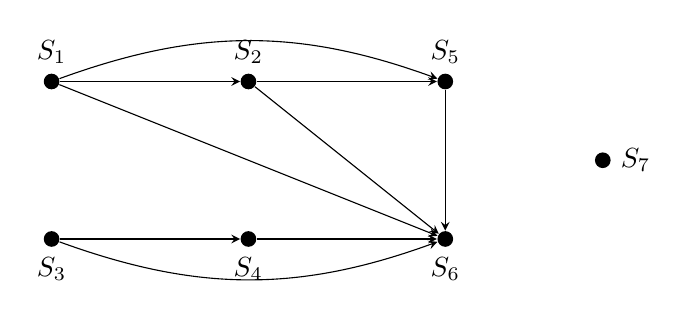
\begin{tikzpicture}[>=stealth, node distance=2.8cm]

% Nodes (top row)
\node (S1) at (0,2) [circle,fill=black,inner sep=2pt,label=above:$S_1$] {};
\node (S2) at (2.5,2) [circle,fill=black,inner sep=2pt,label=above:$S_2$] {};
\node (S5) at (5,2)   [circle,fill=black,inner sep=2pt,label=above:$S_5$] {};

% Nodes (bottom row)
\node (S3) at (0,0) [circle,fill=black,inner sep=2pt,label=below:$S_3$] {};
\node (S4) at (2.5,0) [circle,fill=black,inner sep=2pt,label=below:$S_4$] {};
\node (S6) at (5,0)   [circle,fill=black,inner sep=2pt,label=below:$S_6$] {};

% Isolated node S7
\node (S7) at (7,1) [circle,fill=black,inner sep=2pt,label=right:$S_7$] {};

% Horizontal edges (top)
\draw[->] (S1) -- (S2);
\draw[->] (S2) -- (S5);

% Horizontal edges (bottom)
\draw[->] (S3) -- (S4);
\draw[->] (S4) -- (S6);

% Vertical edge from S5 to S6
\draw[->] (S5) -- (S6);

% Curved edges 
\draw[->, bend left=20] (S1) to (S5);
\draw[->, bend right=20] (S3) to (S6);

% From top to bottom
\draw[->] (S1) to (S6);
\draw[->] (S2) to (S6);

% Curved edges from S3 and S4 to S6


\end{tikzpicture}
\end{center}
}

\item \streasy (Rosen 10.2-6) Show that the sum, over the set of people at a party, of the number of people a person has shaken hands with, is even. Assume that no one shakes their own hand.

\solution{Model the party by a simple (undirected) graph \(G=(V,E)\) whose vertices are the people at the party and where an edge \(\{u,v\}\in E\) means that persons \(u\) and \(v\) have shaken hands. By assumption there are no loops, so no vertex is adjacent to itself.

For each vertex \(v\in V\) let \(\deg(v)\) denote the number of people \(v\) has shaken hands with (the degree of \(v\)). Each handshake corresponds to an edge and contributes exactly \(1\) to the degree of each of its two endpoints. Therefore every edge of \(G\) is counted twice in the sum of the degrees. Hence
\[
\sum_{v\in V}\deg(v)=2|E|.
\]
}

\item \strmedium (Rosen 10.2-18) Show that in a simple graph with at least two vertices there must be two vertices that have the same degree.

\solution{Let \(G\) be a simple graph on \(n\ge 2\) vertices. The degree of any vertex lies in the set
\[
\{0,1,2,\dots,n-1\}.
\]
Thus there are \(n\) vertices and \(n\) possible degree values. However, a simple graph cannot simultaneously have a vertex of degree \(0\) (an isolated vertex) and a vertex of degree \(n-1\) (a vertex adjacent to all others), because if some vertex has degree \(n-1\) then no vertex can be isolated. Hence the set of possible degrees that actually occur in \(G\) is contained in either
\[
\{0,1,\dots,n-2\}\quad\text{or}\quad\{1,2,\dots,n-1\},
\]
each of which has only \(n-1\) distinct values.

By the pigeonhole principle, \(n\) vertices distributed among at most \(n-1\) possible degree values force at least two vertices to share the same degree. Therefore \(G\) has two distinct vertices with equal degree.

We already saw this exercise with computers network! In fact, it can take many forms :)
}

\item \strhard (Rosen 10.2-26) For which values of \(n\) are the following graphs bipartite?
\begin{enumerate}[a)]
  \item \(K_n\) (the complete graph on \(n\) vertices),
  \item \(C_n\) (the cycle on \(n\) vertices),
  \item \(W_n\) (the wheel on \(n\) vertices; i.e. a vertex (hub) joined to every vertex of a cycle \(C_{n-1}\)),
  \item \(Q_n\) (the \(n\)-dimensional hypercube graph).
\end{enumerate}

\solution{\begin{enumerate}[a)]
\item \(\;K_n\) is bipartite \(\iff n\le 2\).

\begin{proof}
(\(\Rightarrow\)) Assume \(K_n\) is bipartite. Then its vertex set can be
partitioned into two parts \(V_1\) and \(V_2\) so that no edge has both endpoints
in the same part. But in the complete graph \(K_n\) every two distinct
vertices are adjacent. Hence each of the parts \(V_1\) and \(V_2\) can contain at
most one vertex. Therefore
\[
n=|V(K_n)|=|V_1|+|V_2|\le 1+1=2,
\]
so \(n\le2\).

(\(\Leftarrow\)) If \(n\le2\) then \(K_n\) is either a single vertex \(K_1\) or
a single edge \(K_2\). Both are bipartite: for \(K_1\) take the partition
\(\{ \{v\},\varnothing\}\), and for \(K_2\) take the partition consisting of
the two endpoints as the two parts. Thus \(K_n\) is bipartite when \(n\le2\).

\end{proof}

{\em Alternative proof (using cycles):}
A bipartite graph has no odd cycle. For \(n\ge 3\), \(K_n\) contains a triangle \(K_3\), so it is not bipartite. The graphs \(K_1\) and \(K_2\) are trivially bipartite (one vertex, and an edge joining two partite sets, respectively).\qed


\item \(\;C_n\) is bipartite \(\iff n\) is even.

\begin{proof}
Label the vertices of \(C_n\) in cyclic order as
\[
v_0,v_1,\dots,v_{n-1}
\]
and write indices modulo \(n\), so edges are exactly the pairs
\(v_i v_{i+1}\) for \(i=0,1,\dots,n-1\).

$(\Rightarrow)$  
Assume \(n\) is even and define
\[
V_1=\{v_i:\; i\text{ is even}\},\qquad V_2=\{v_i:\; i\text{ is odd}\}.
\]
Every edge \(v_i v_{i+1}\) joins an even-indexed vertex to an odd-indexed vertex,
so no edge has both endpoints in \(V_1\) and no edge has both endpoints in \(V_2\).
Thus \(V(C_n)=V_1\cup V_2\) is a partition into two independent sets, so \(C_n\)
is bipartite.

$(\Leftarrow)$  
Suppose \(C_n\) is bipartite with vertex partition \(V= V_1\dot\cup V_2\). Place
\(v_0\) in \(V_1\) (renaming the parts if necessary). Since \(v_0\) is adjacent
to \(v_1\), we must have \(v_1\in V_2\); then \(v_2\) is adjacent to \(v_1\) so
\(v_2\in V_1\); continuing in this way we obtain for every \(k\)
\[
v_k\in V_1\iff k\text{ is even},\qquad v_k\in V_2\iff k\text{ is odd}.
\]
In particular \(v_n\) must lie in the same part as \(v_0\). But \(v_n=v_0\) and
after \(n\) steps the parity of the index flips exactly when \(n\) is odd.
 If \(n\) were odd we would get
\(v_n\in V_2\) while \(v_n=v_0\in V_1\), a contradiction. Therefore \(n\) is even.
\end{proof}


{\em Alternative proof (using coloring):}
A cycle is bipartite exactly when it has even length: if \(n\) is even we can 2-colour the vertices alternately around the cycle, whereas if \(n\) is odd the cycle is an odd cycle and hence not bipartite.\qed


\item \(\;W_n\) is not bipartite for all  \(n\ge 3\).

\begin{proof}
The Wheel Graph $W_n$ has the vertex set $V = \{v_0, v_1, v_2, \ldots, v_n\}$, where $v_0$ is the {\em central hub} and $v_1, \ldots, v_n$ form an $n$-cycle, $C_n$. The edges include the $n$ {\em spokes} $(v_0, v_i)$ for $i=1, \ldots, n$, and the $n$ {\em cycle edges} $(v_i, v_{i+1})$ for $i=1, \ldots, n-1$, plus $(v_n, v_1)$.


Assume $W_n$ is bipartite for some $n \ge 3$.
 If $W_n$ is bipartite, its vertex set $V$ can be partitioned into two disjoint sets, $V_1$ and $V_2$.
 %
 Consider the hub vertex, $v_0$. Without loss of generality, assume that $v_0 \in V_1$.
%
Since $v_0$ is connected by an edge (a spoke) to every other vertex $v_i$ ($i=1, \ldots, n$), it must be the case that $V_2 = \{v_1, v_2, \ldots, v_n\} $.
    
Now, consider the cycle $C_n$ formed by the vertices $v_1, v_2, \ldots, v_n$. Since $n \ge 3$, the edge $(v_1, v_2)$ connects two vertices both belonging to the same set, $V_2$. ABSURD!

\end{proof}


{\em Alternative proof (using cycles):}
By definition \(W_n\) contains a copy of a cycle \(C_{n-1}\) together with a hub joined to every vertex of that cycle. Whenever \(C_{n-1}\) has at least three vertices (the usual wheel requires \(n-1\ge 3\), i.e. \(n\ge 4\)), the hub together with any two adjacent vertices of the cycle forms a triangle. Thus \(W_n\) contains an odd cycle and so is not bipartite. (For the degenerate small values \(n\le 3\) the wheel is either undefined or reduces to small complete graphs which also are not bipartite except \(K_1\) or \(K_2\) as above.)\qed

\item \(\;Q_n\) is bipartite for every integer \(n\ge 1\).

\begin{proof}
We proceed by induction on \(n\).

\textbf{Base case.} \(Q_1\) is just \(K_2\), which is bipartite (its two endpoints form the two partite sets).

\textbf{Inductive step.} Assume \(Q_n\) is bipartite for some \(n\ge 1\).  
Construct \(Q_{n+1}\) as follows: take two disjoint copies \(Q_n^{(0)}\) and \(Q_n^{(1)}\) of \(Q_n\), and join each vertex of \(Q_n^{(0)}\) to the corresponding vertex of \(Q_n^{(1)}\) by a single edge. (This is the standard construction of \(Q_{n+1}\) as the Cartesian product \(Q_n\times K_2\).)

By the inductive hypothesis \(Q_n\) has a bipartition \(V_1\cup V_2\). Use this partition for the first copy \(Q_n^{(0)}\). For the second copy \(Q_n^{(1)}\) use the \emph{swapped} partition \(V_2\cup V_1\) (so a vertex that lies in \(V_1\) in the first copy is placed in the opposite part in the second copy). Now check edges:
\begin{itemize}
  \item Any edge internal to \(Q_n^{(0)}\) joins a vertex in \(V_1\) to one in \(V_2\) by the bipartiteness of \(Q_n\).
  \item Any edge internal to \(Q_n^{(1)}\) joins a vertex in \(V_2\) to one in \(V_1\) (since we swapped the parts), so it also joins the two different parts.
  \item Each edge joining corresponding vertices of the two copies connects a vertex in \(V_1\) (in one copy) with the corresponding vertex placed in \(V_2\) (in the other copy), hence also joins different parts.
\end{itemize}
Thus all edges of \(Q_{n+1}\) join the two partite sets, so \(Q_{n+1}\) is bipartite.

By induction, \(Q_n\) is bipartite for all \(n\ge 1\).
\end{proof}
\end{enumerate}}

%\item \strhard (Rosen 10.2-27) Suppose that there are four employees in the computer support group of the School of Engineering of a large university. Each employee will be assigned to support one of four different areas: hardware, software, networking, and wireless. Suppose that Ping is qualified to support hardware, networking, and wireless; Quiggley is qualified to support software and networking; Ruiz is qualified to support networking and wireless, and Sitea is qualified to support hardware and software.
%\begin{itemize}
%\item[a)] Use a bipartite graph to model the four employees and
%their qualifications.
%\item[b)] Use Hall's theorem to determine whether there is an
%assignment of employees to support areas so that each
%employee is assigned one area to support.
%\item[c)] If an assignment of employees to support are as so that each employee is assigned to one support area exists, find one.
%\end{itemize}
%\solution{
%\begin{itemize}
%\item[a)]  The bipartite graph has vertices $h, s, n, w$ representing the support areas and $P, Q, R, S$ representing the employees. The qualifications are modeled by the bipartite graph with edges $P_h, P_n, P_w, Q_s, Q_n, R_n, R_w, S_h, S_s$.
%\item[b)] Since every vertex representing an area has degree at least 2, the condition in Hall's theorem is satisfied for sets of size less than 3. We can easily check that the number of employees qualified for each of the four subsets of size 3 is at least 3, and clearly the number of employees qualified for each of the subsets of size 4 has size 4.
%\item[c)] The answer is not unique; one complete matching is $\{P_n, Q_s, R_w, S_h\}$, which is easily found by inspection.
%\end{itemize}
%}

\item  \streasy (Rosen 10.2-38) The degree sequence of a graph is the sequence of the degrees of the vertices of the graph in non-increasing order.  What is the degree sequence of the bipartite graph $K_{m,n}$ where $m$ and $n$ are positive integers? Explain your answer.

\solution{
The bipartite graph \(K_{m,n}\) has two partite sets: one with \(m\) vertices and one with \(n\) vertices. Every vertex in the first part is adjacent to all \(n\) vertices in the second part, and every vertex in the second part is adjacent to all \(m\) vertices in the first part. There are no edges within each partite set.

Therefore:
\begin{itemize}
    \item each of the \(m\) vertices in the first part has degree \(n\),
    \item each of the \(n\) vertices in the second part has degree \(m\).
\end{itemize}

Arranging these degrees in non-increasing order gives the degree sequence
\[
(\underbrace{\max(m,n),\ldots,\max(m,n)}_{\min(m,n)\text{ times}},\;
 \underbrace{\min(m,n),\ldots,\min(m,n)}_{\max(m,n)\text{ times}}).
\]

}

%\item \streasy (Rosen 10.2-39) What is the degree sequence of $K_n$, where $n$ is a positive
%integer? Explain your answer.
%\solution{
%Each of the n vertices is adjacent to each of the other $n - 1$ vertices, so the degree sequence is simply $n - 1, n - 1, \ldots , n - 1$, with $n$ terms in the sequence.
%}

\item \strmedium (Rosen 10.2-53) A simple graph is called {\em regular} if every vertex of this graph has the same degree. %A regular graph is called $n-$regular if every vertex in this graph has degree $n$.
For which values of $n$ are these graphs regular?

a) $K_n$ \qquad b) $C_n$  \qquad c) $W_n$  \qquad d) $Q_n$

\solution{
\begin{itemize}
\item[a)] The complete graph $K_n$ is regular for all values of $n \geq 1$, since the degree of each vertex is $n - 1$.
\item[b)] The degree of each vertex of $C_n$ is 2 for all $n$ for which $C_n$ is defined, namely $n \geq 3$, so $C_n$ is regular for all these values of $n$.
\item[c)] The degree of the middle vertex of the wheel $W_n$ is $n$, and the degree of the vertices on the ``rim'' is 3. Therefore $W_n$ is regular if and only if $n = 3$. Of course $W_3$ is the same as $K_4$ .
\item[d)] The cube $Q_n$ is regular for all values of $n\geq 0$, since the degree of each vertex in $Q_n$ is $n$. (Note that $Q_0$ is the graph with 1 vertex.)
\end{itemize}
}

\item  \streasy (Rosen 10.2-54) For which values of $m$ and $n$ is $K_{m,n}$ regular?

\solution{
A graph is regular if all of its vertices have the same degree.
Thus \(K_{m,n}\) is regular precisely when the degrees of the two parts are equal; that is,
$
m = n.
$
}

\item \streasy (Rosen 10.2-59) The complementary graph $\ov{G}$ of a simple graph $G$ has the same vertices as $G$. Two vertices are adjacent in $\ov{G}$ if and only if they are not adjacent in $G$. Describe each of these graphs.

a) $\ov{K_n}$ \qquad b) $\ov{K_{m,n}}$  \qquad c) $\ov{C_n}$  \qquad d) $\ov{Q_n}$

\solution{\begin{enumerate}[a)]
    \item The complement of a complete graph is a graph with no edges.

    \item Since all the edges between the parts are present in \(K_{m,n}\), but none of the edges between vertices in the same part are, the complement must consist precisely of the disjoint union of a \(K_m\) and a \(K_n\); that is, the graph containing all the edges joining two vertices in the same part and no edges joining vertices in different parts.

    \item There is really no better way to describe this graph than simply by saying it is the complement of \(C_n\). One representation would be to take as vertex set the integers from \(1\) to \(n\), inclusive, with an edge between distinct vertices \(i\) and \(j\) whenever \(i\) and \(j\) do \emph{not} differ by \(\pm 1\), modulo \(n\).

    \item Again, there is really no better way to describe this graph than simply by saying it is the complement of \(Q_n\). One representation would be to take as vertex set the bit strings of length \(n\), with two vertices joined by an edge if the bit strings differ in more than one bit.
\end{enumerate}}

\item \streasy (Rosen 10.3-9) Represent each of these graphs with an adjacency matrix.

a) $K_4$ \qquad b) $K_{1,4}$  \qquad c) $K_{2,3}$  \qquad d) $C_4$ \qquad e) $W_4$ \qquad f) $Q_3$

\solution{We can solve these problems by first drawing the graph, then labeling the vertices, and finally constructing the matrix by putting a 1 in position $(i,j)$ whenever vertices $i$ and $j$ are joined by an edge. It helps to choose a nice order, since then the matrix will have nice patterns in it.
\begin{enumerate}[a)]
\item The order of the vertices does not matter, since they all play the same role. The matrix has $0$'s on the diagonal, since there are no loops in the complete graph.
\[
\begin{bmatrix}
0 & 1 & 1 & 1 \\
1 & 0 & 1 & 1 \\
1 & 1 & 0 & 1 \\
1 & 1 & 1 & 0
\end{bmatrix}
\]
\item  We put the vertex in the part by itself first.
\[
\begin{bmatrix}
0 & 1 & 1 & 1 & 1 \\
1 & 0 & 0 & 0 & 0 \\
1 & 0 & 0 & 0 & 0\\
1 & 0 & 0 & 0 & 0 \\
1 & 0 & 0 & 0 & 0 
\end{bmatrix}
\]
\item  We put the vertices in the part of size 2 first. Notice the block structure. 
\[
\begin{bmatrix}
0 & 0 & 1 & 1 & 1 \\
0 & 0 & 1 & 1 & 1 \\
1 & 1 & 0 & 0 & 0\\
1 & 1 & 0 & 0 & 0 \\
1 & 1 & 0 & 0 & 0 
\end{bmatrix}
\]

\item  We put the vertices in the same order in the matrix as they are around the cycle.
\[
\begin{bmatrix}
0 & 1 & 0 & 1 \\
1 & 0 & 1 & 0 \\
0 & 1 & 0 & 1 \\
1 & 0 & 1 & 0
\end{bmatrix}
\]

\item  We put the center vertex first. Note that the last four columns of the last four rows represent a $C_4$.
\[
\begin{bmatrix}
0 & 1 & 1 & 1 & 1 \\
1 & 0 & 1 & 0 & 1 \\
1 & 1 & 0 & 1 & 0\\
1 & 0 & 1 & 0 & 1 \\
1 & 1 & 0 & 1 & 0 
\end{bmatrix}
\]
\item  We can label the vertices by the binary numbers from 0 to 7. Thus the first row (also the first column) of this matrix corresponds to the string 000, the second to the string 001, and so on. Since $Q_3$ has 8 vertices, this is an $8 \times 8$ matrix.
\[
\begin{bmatrix}
0 & 1 & 1 & 0 & 1 & 0 & 0 & 0 \\
1 & 0 & 0 & 1 & 0 & 1 & 0 & 0\\
1 & 0 & 0 & 1 & 0 & 0 & 1 & 0\\
0 & 1 & 1 & 0 & 0 & 0 & 0 & 1 \\
1 & 0 & 0 & 0 & 0 & 1 & 1 & 0 \\
0 & 1 & 0 & 0 & 1 & 0 & 0 & 1 \\
0 & 0 & 1 & 0 & 1 & 0 & 0 & 1 \\
0 & 0 & 0 & 1 & 7 & 1 & 1 & 0
\end{bmatrix}
\]
\end{enumerate}}

\item  \streasy (Rosen 10.3-25) Is every zero-one square matrix that is symmetric and has zeros on the diagonal the adjacency matrix of a simple graph?

\solution{
Since the matrix is symmetric, it has to be square, so it represents a graph of some sort. In fact, such a matrix does represent a simple graph. The fact that it is a zero-one matrix means that there are no parallel edges. The fact that there are 0's on the diagonal means that there are no loops. The fact that the matrix is symmetric means that the edges can be assumed to be undirected. Hence the answer to this question is ``yes.''
}

\item \strmedium (Rosen 10.3-28) What is the sum of the entries in a row of the adjacency matrix for an undirected graph? For a directed graph?
\solution{
In an undirected graph,, the sum of the entries in row $i$ of the adjacency
matrix is the degree of the vertex $v_i$.
In a directed graph, the sum of the entries in row $i$ of the adjacency 
matrix is the outdegree of the vertex $v_i$. 

}

\item \strhard (Rosen 10.3-29) What is the sum of the entries in a column of the adjacency matrix for an undirected graph? For a directed graph?
\solution{
In an undirected graph, each edge incident to a vertex $j$ contributes 1 in the $j^{th}$ column; thus the sum of the entries in that column is just the number of edges incident to $j$. Another way to state the answer is that the sum of the entries is the degree of $j$ minus the number of loops at $j$, since each loop contributes 2 to the degree count.
In a directed graph, each edge whose terminal vertex is $j$ contributes 1 in the $j^{th}$ column; thus the sum of the entries in that column is just the number of edges that have $j$ as their terminal vertex. Another way to state the answer is that the sum of the entries is the in-degree of $j$.
}

\item \strhard (Rosen 10.3-50) A simple graph $G$ is called {\em self-complementary} if $G$ and $\ov{G}$ are isomorphic.
 Show that the graph below is self-complementary.
 \begin{center}
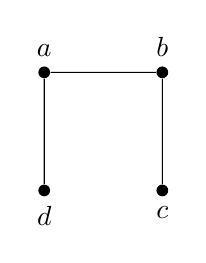
\begin{tikzpicture}[scale=1.5]
    \node (d) at (0,0) [circle,fill=black,inner sep=1.5pt,label=below:$d$] {};
    \node (c) at (1,0) [circle,fill=black,inner sep=1.5pt,label=below:$c$] {};
    \node (b) at (1,1) [circle,fill=black,inner sep=1.5pt,label=above:$b$] {};
    \node (a) at (0,1) [circle,fill=black,inner sep=1.5pt,label=above:$a$] {};

    \draw (d) -- (a) -- (b) -- (c) ;
\end{tikzpicture}
\end{center}
\solution{
The graph \(G\) has vertices \(a,b,c,d\) and edges
\[
E(G)=\{da,\; ab,\; bc\}.
\]
Since \(K_4\) has \(6\) edges and \(G\) has \(3\) edges, the complement
\(\overline{G}\) also has \(3\) edges. The missing edges are
\[
E(\overline{G})=\{dc,\; db,\; ac\}.
\]

To show that \(G\) is self-complementary, we exhibit an isomorphism
\(\varphi : V(G)\to V(G)\) such that
\[
uv\in E(G) \quad\Longleftrightarrow\quad \varphi(u)\varphi(v)\in E(\overline{G}).
\]

Consider the permutation
\[
\varphi = (a\ c)(b\ d),
\]
that is,
\[
\varphi(a)=c,\qquad \varphi(c)=a,\qquad
\varphi(b)=d,\qquad \varphi(d)=b.
\]

We check that each edge of \(G\) is mapped to an edge of \(\overline{G}\):

\[
da \mapsto \varphi(d)\varphi(a)=bc \in E(\overline{G}),
\]
\[
ab \mapsto \varphi(a)\varphi(b)=cd \in E(\overline{G}),
\]
\[
bc \mapsto \varphi(b)\varphi(c)=da \in E(\overline{G}).
\]

Thus, \(\varphi\) is a bijection that maps edges of \(G\) to edges of
\(\overline{G}\), showing that
\[
G \cong \overline{G}.
\]

Therefore, the graph is \emph{self-complementary}.
}

\item  \strhard (Rosen 10.3-53) For which integers $n$ is $C_n$ self-complementary?
\solution{
If $C_n$ is to be self\mbox{-}complementary, then $C_n$ must have the same number of edges as its complement. We know that $C_n$ has $n$ edges. Its complement has the number of edges in $K_n$ minus the number of edges in $C_n$, namely
\[
\binom{n}{2} - n = \frac{n(n-1)}{2} - n.
\]
If we set these two quantities equal, we obtain
\[
\frac{n(n-1)}{2} - n = n,
\]
which has $n = 5$ as its only solution. Thus $C_5$ is the only $C_n$ that \emph{might} be self\mbox{-}complementary -- our argument just shows that it has the same number of edges as its complement, not that it is indeed isomorphic to its complement. However, if we draw $C_5$ and then draw its complement, we see that the complement is again a copy of $C_5$. Thus $n = 5$ is the answer to the problem.
}

\item \streasy (Rosen 10.4-16) Suppose that $G = (V , E)$ is a directed graph. A vertex $w \in V$ is {\em reachable} from a vertex $v \in V$ if there is a directed path from $v$ to $w$. The vertices $v$ and $w$ are {\em mutually reachable} if there are both a directed path from $v$ to $w$ and a directed path from $w$ to $v$ in $G$. Show that if $G=(V,E)$ is a directed graph and $u,v, w$ are vertices in $V$ for which $u$ and $v$ are mutually reachable and $v$ and $w$ are mutually reachable, then $u$ and $w$ are mutually reachable.

\solution{Let \(G=(V,E)\) be a directed graph and let \(u,v,w\in V\).  
Assume \(u\) and \(v\) are mutually reachable and \(v\) and \(w\) are mutually reachable.  By definition this means there is a directed path from \(u\) to \(v\), a directed path from \(v\) to \(u\), a directed path from \(v\) to \(w\), and a directed path from \(w\) to \(v\).

Write the path from \(u\) to \(v\) as
\[
P=(u=x_0,x_1,\dots,x_k=v)
\]
and the path from \(v\) to \(w\) as
\[
Q=(v=y_0,y_1,\dots,y_m=w).
\]
Concatenating \(P\) and \(Q\) at the common vertex \(v\) gives the directed path
\[
P\cdot Q=(u=x_0,x_1,\dots,x_k=v=y_0,y_1,\dots,y_m=w)
\]
from \(u\) to \(w\). Thus there is a directed path \(u\to w\).

Similarly, let \(P'=(v=z_0,z_1,\dots,z_{k'}=u)\) be the path from \(v\) to \(u\) and \(Q'=(w=t_0,t_1,\dots,t_{m'}=v)\) the path from \(w\) to \(v\).  Concatenating \(Q'\) and \(P'\) at \(v\) yields a directed path
\[
Q'\cdot P'=(w=t_0,t_1,\dots,t_{m'}=v=z_0,z_1,\dots,z_{k'}=u)
\]
from \(w\) to \(u\). Hence there is a directed path \(w\to u\).

Since we have both \(u\to w\) and \(w\to u\), the vertices \(u\) and \(w\) are mutually reachable.
}

\item \strmedium (Rosen 10.4-17) Show that if $G = (V , E)$ is a directed graph, then the strong components of two vertices $u$ and $v$ of $V$ are either the same or disjoint. [Hint: Use the last exercise.]

\solution{The hardest part of this exercise is figuring out what we need to prove.  
It is enough to prove that if the strong components of \(u\) and \(v\) are not disjoint, then they are the same.

So suppose that \(w\) is a vertex that is in both the strong component of \(u\) and the strong component of \(v\).  
(It is enough to consider the vertices in these components, because the edges in a strong component are just all the edges joining the vertices in that component.)

This means that there are directed paths (in each direction) between \(u\) and \(w\) and between \(v\) and \(w\).  
It follows that there are directed paths from \(u\) to \(v\) and from \(v\) to \(u\), via \(w\).

Suppose \(x\) is a vertex in the strong component of \(u\).  
Then \(x\) is also in the strong component of \(v\), because there is a path from \(x\) to \(v\) (namely, the path from \(x\) to \(u\) followed by the path from \(u\) to \(v\)) and vice versa.
}

\item \strmedium (Rosen 10.4-19) Find the number of paths of length $n$ between two different vertices in $K_4$ if $n$ is

a) 2. \qquad b) 3.\qquad c) 4.\qquad d) 5.

\solution{One approach here is simply to invoke Theorem 2 and take successive powers of the adjacency matrix
\[
\begin{bmatrix}
0 & 1 & 1 & 1  \\
1 & 0 & 1 & 1  \\
1 & 1 & 0 & 1 \\
1 & 1 & 1 & 0  \\ 
\end{bmatrix}
\]
The answers are the off-diagonal elements of these powers. An alternative approach is to argue combinatorially as follows. Without loss of generality, we assume that the vertices are called \(1,2,3,4\), and the path is to run from \(1\) to \(2\). A path of length \(n\) is determined by choosing the \(n-1\) intermediate vertices. Each vertex in the path must differ from the one immediately preceding it.
\begin{enumerate}[a)]
\item  A path of length \(2\) requires the choice of \(1\) intermediate vertex, which must be different from both of the ends. Vertices \(3\) and \(4\) are the only ones available. Therefore the answer is \(2\).

\item  Let the path be denoted \(1,x,y,2\).  
If \(x=2\), then there are \(3\) choices for \(y\).  
If \(x=3\), then there are \(2\) choices for \(y\); similarly if \(x=4\).  
Therefore there are \(3 + 2 + 2 = 7\) possibilities in all.

\item  Let the path be denoted \(1,x,y,z,2\).  
If \(x=3\), then by part (b) there are \(7\) choices for \(y\) and \(z\).  
Similarly if \(x=4\).  
If \(x=2\), then \(y\) and \(z\) can be any two distinct members of \(\{1,3,4\}\), and there are  
\[
P(3,2)=6
\]
ways to choose them.  
Therefore there are \(7+7+6=20\) possibilities in all.

\item  Let the path be denoted \(1,w,x,y,z,2\).  
If \(w=3\), then by part (c) there are \(20\) choices for \(x,y,z\).  
Similarly if \(w=4\).  
If \(w=2\), then \(x\) must be different from \(2\), and there are \(3\) choices for \(x\).  
For each of these there are, by part (b), \(7\) choices for \(y\) and \(z\).  
This gives a total of \(21\) possibilities in this case.  
Therefore the answer is  
\[
20 + 20 + 21 = 61.
\]
\end{enumerate}
}

\item \strhard (Rosen 10.4-28)  Show that every connected graph with $n$ vertices has at least $n - 1$ edges.
\solution{ By induction in $n$.
For \(n=1\) the claim is trivial. Assume as an induction hypothesis that every
connected graph on \(n-1\) vertices has at least \(n-2\) edges. Now let \(G\) be
a connected graph on \(n\) vertices, and remove any vertex \(v\).

If \(G - v\) is connected, then by the induction hypothesis it has at least
\(n-2\) edges. Since \(G\) is connected, the removed vertex \(v\) must have had
at least one incident edge in \(G\). Therefore
\[
|E(G)| \;\ge\; (n-2) + 1 \;=\; n-1.
\]

If \(G - v\) is disconnected, then it has at least two components. Because \(G\)
was connected, the vertex \(v\) must have at least one neighbor in each
component, so it contributes at least two incident edges. Hence
\[
|E(G)| \;\ge\; (n-2) + 2 \;>\; n-1.
\]

In either case we conclude that every connected graph on \(n\) vertices has at
least \(n-1\) edges.

}
\item \strmedium (Rosen 10.4-29)  Let $G = (V,E)$ be a simple graph. Let $R$ be the relation on $V$ consisting of pairs of vertices $(u, v)$ such that there is a path from $u$ to $v$ or such that $u = v$. Show that $R$ is an equivalence relation.
\solution{The definition given here makes it clear that $u$ and $v$ are related if and only if they are in the same component. In other words $f(u) = f(v)$ where $f(x)$ is the component in which $x$ lies. Therefore by Exercise 9 in Section 9.5 this is an equivalence relation.}
\end{enumerate}

\end{document}

